\section{The Cost of Modularity, and the Surprise of Autonomy}
\label{sec_disc_modularity_autonomy}

The third cross-cutting finding concerns the cost of separating grouping
from detection and the behaviour of the resulting autonomous pipeline.
Unlike HigherHRNet's associative-embedding (AE) head,
PG-GAT is trained as a separate grouping module and operates only on
detected keypoints.
This separation provides detector independence,
but removes the joint-training advantage available to a grouping
representation that is learned together with the detector.
On the HigherHRNet end-to-end evaluation, the consequence is measurable -
the oracle-$K$ PG-GAT pipeline reaches $0.9591$ PGA compared with
$0.9847$ for HigherHRNet's native AE grouping on the same matched
detections,
a difference of $0.0256$.

This gap is an expected consequence of the modular design.
The AE tags are learned alongside the keypoint heatmaps and can adapt
directly to the detector features and errors encountered during training.
PG-GAT, by contrast, receives only the resulting keypoint coordinates,
joint types,
and associated node features.
It has no access to the detector's intermediate representation and cannot
influence which keypoints are produced.
The comparison therefore measures a trade-off rather than a failure to
reproduce the AE architecture -
PG-GAT gives up some grouping accuracy in exchange for a grouping
representation that can be applied independently of the detector that
produced the keypoints.

The detector-swap experiments make this interpretation stronger than
the HigherHRNet comparison alone.
The same frozen PG-GAT checkpoint and K-head can be applied to
HigherHRNet,
YOLO11x-pose,
and RTMO-L without retraining,
and the autonomous grouping result remains approximately $0.02$ below
each detector's native assignment.
The stability of this difference across three detector families
suggests that the measured cost is associated with the modular grouping
formulation rather than with a particular interaction between PG-GAT
and HigherHRNet.
The benefit being purchased is correspondingly concrete -
the grouping network can be reused when the upstream detector changes.

The second part of the result is less intuitive.
Replacing the ground-truth person count $K$ with the prediction of the
frozen-backbone K-head might be expected to introduce another source
of error.
Instead, the autonomous HigherHRNet pipeline reaches $0.9644$ PGA,
compared with $0.9591$ when $k$-means is supplied with the ground-truth
$K$.
The difference is small,
but its direction is consistent with the detector-swap experiments,
which makes an explanation beyond random variation in a
single evaluation worth considering.

The key distinction is between the number of people annotated in the
image and the number of people represented by the detections that
actually reach the grouping stage.
These quantities are identical when ground-truth keypoints are used,
but they need not remain identical after detection and matching.
HigherHRNet recovers only a subset of the annotated keypoints under the
evaluation protocol.
A person may therefore be present in the ground truth while contributing
too few, or no, matched detections to form a meaningful cluster.
Supplying the annotation-level $K$ to $k$-means nevertheless forces the
algorithm to produce that many clusters from the incomplete detection set.

This creates what can be viewed as a phantom-cluster effect.
When the specified $K$ is larger than the number of people effectively
represented in the detected embeddings,
$k$-means must allocate additional centroids somewhere.
These centroids can split the detections of a well-represented person
rather than recover a person whose keypoints are absent.
The ground-truth value is therefore an oracle for the original image,
but not necessarily an oracle for the incomplete representation
presented to the grouping algorithm.

The learned K-head operates on that incomplete representation instead.
Its prediction is derived from pooled PG-GAT embeddings and the observed
keypoint count,
so it can implicitly adapt to the number of people that remain
represented after detection.
Its $76.1\%$ exact-$K$ accuracy therefore does not tell the complete
story -
a prediction that differs from the annotation-level count can still
provide a better value for partitioning the detected subset.
In this setting, being "wrong" against the annotated $K$ can be useful
if the prediction is closer to the effective number of recoverable people.

This interpretation is supported by the detector-swap results.
As detector recall decreases, the advantage of predicted $K$ over
oracle $K$ increases,
$+0.0006$ for YOLO11x-pose at $0.816$ recall,
$+0.0053$ for HigherHRNet at $0.793$,
and $+0.0304$ for RTMO-L at $0.774$.
In the ground-truth-keypoint control, where the keypoint set is
complete and the annotation-level $K$ is genuinely the correct
partition size, predicted $K$ instead carries a penalty.
The pattern is therefore consistent with the effective-person-count
explanation,
K-estimation becomes useful not because it predicts the annotation
more accurately than the oracle,
but because it adapts the clustering problem to the information that
survives detection.

The two halves of the finding are consequently related.
Detector independence introduces a modest grouping cost because PG-GAT
gives up joint optimisation with the detector,
but operating on detached detections also changes what the appropriate
person count means.
Once the detector produces an incomplete representation of the scene,
the annotation-level $K$ is no longer necessarily the best value for
clustering that representation.
The autonomous pipeline can therefore outperform its oracle-$K$
diagnostic while remaining fully independent of ground truth at inference.
The following sections examine the modularity cost and this
effective-person-count mechanism in more detail.

\subsection{The 0.0256 detector-independence gap}
\label{sec_disc_modularity_autonomy_gap}

The end-to-end evaluation of Section~\ref{sec_res_e2e} provides the
clearest measurement of the cost introduced by separating grouping from
detection.
On the matched HigherHRNet detections, the detector's native
associative-embedding (AE) grouping reaches $0.9847$ PGA,
while the headline PG-GAT configuration reaches $0.9591$ with oracle $K$.
The difference is $0.0256$.
This gap also narrows consistently as the PG-GAT pipeline is improved,
the synthetic-only two-layer configuration trails AE by $0.1081$,
the legacy COCO fine-tune reduces the difference to $0.0417$,
and the sweep-selected architecture and fine-tune recipe reduce it
further to $0.0256$.

The detector-swap experiment of Section~\ref{sec_res_e2e_swap} shows
that this behaviour is not specific to HigherHRNet.
The same frozen PG-GAT checkpoint and K-head are applied zero-shot to
detections from YOLO11x-pose and RTMO-L,
despite neither detector contributing training data to the grouping module.
The autonomous pipeline trails their native person assignments by
$0.0210$ and $0.0220$ PGA respectively,
compared with $0.0203$ for the autonomous HigherHRNet configuration.
The similarity of these gaps across three detector families is stronger
evidence for the modularity claim than the HigherHRNet result alone -
changing the upstream detector does not require the grouping network
to be retrained,
and the measured cost remains close to $0.02$ PGA.

A likely reason for the remaining gap is the advantage available to a
jointly trained grouping representation.
HigherHRNet learns its AE tags together with the keypoint detector on
the COCO training distribution.
The tag representation can therefore adapt to the same intermediate
features and image statistics used to produce the heatmaps.
PG-GAT does not have access to this information.
It operates after detection and must infer person identity from the
resulting keypoint representation,
which deliberately removes the dependency on detector-specific internal
features.
The two approaches consequently solve the grouping problem under
different information constraints.

This distinction is also important when interpreting the parameter
counts.
HigherHRNet's AE tag head contains only approximately $561$ parameters,
whereas the sweep-selected PG-GAT contains $333{,}552$.
PG-GAT therefore does not obtain its modularity through a smaller
grouping model.
The advantage is architectural separation.
The AE tag head forms part of a representation learned jointly with the
HigherHRNet backbone and is not, in the form evaluated here,
a standalone grouping module that can simply be transferred to the
output of another detector.
PG-GAT instead accepts detected keypoints through a detector-independent
interface,
which is what permits the same frozen checkpoint to operate on
HigherHRNet,
YOLO11x-pose,
and RTMO-L.

The comparison should therefore be understood as a trade-off in
capability rather than as a claim that PG-GAT is uniformly preferable
to AE.
On HigherHRNet detections, native AE grouping provides the higher PGA.
If the detector is fixed and the complete detection-and-grouping
pipeline can be trained jointly, there is little reason on the evidence
of this work to give up that advantage.
In such a setting, the native grouping mechanism is both more accurate
and substantially smaller than PG-GAT.

The situation changes when the grouping component must remain
independent of the detector.
The detector-swap results demonstrate that PG-GAT can be placed behind
three different keypoint detectors without retraining its embedding
network,
while remaining approximately $0.02$ PGA below each detector's native
assignment.
This capability cannot be inferred from the HigherHRNet comparison alone -
it is directly demonstrated by the zero-shot detector swaps.
The additional PG-GAT parameters and the remaining accuracy difference
are therefore the measured costs of maintaining a separately trainable
and reusable grouping component.

Whether that trade is worthwhile depends on the deployment setting.
For a fixed detector whose native grouping mechanism is available and
can be retained, the results favour the native approach.
For a system in which detectors may be exchanged,
upgraded,
or developed independently of the grouping stage,
the modular PG-GAT interface provides a capability that the coupled
alternatives evaluated here do not provide.
The experimental contribution is therefore not that PG-GAT removes the
cost of decoupling
but that it quantifies that cost -
approximately $0.020$--$0.022$ PGA for the autonomous pipeline across the three detector families
tested,
in exchange for zero-shot reuse of the same grouping network.


\subsection{Why predicted K exceeds oracle K}
\label{sec_disc_modularity_autonomy_autonomy}

The autonomous evaluation of Section~\ref{sec_res_e2e} produces a
counter-intuitive result.
Using the K-head prediction gives an end-to-end PGA of $0.9644$,
compared with $0.9591$ when $k$-means is given the ground-truth person
count.
This occurs even though the K-head predicts the exact ground-truth $K$
in only $76.1\%$ of cases ($91.9\%$ within one person).
If ground-truth $K$ were always the correct number of clusters for the
data presented to $k$-means - an imperfect estimate should reduce
grouping accuracy.
The fact that it does not suggests that the relevant cluster count
changes once detection errors are introduced.

The distinction is between the number of people annotated in the image
and the number represented in the detected keypoints.
HigherHRNet recovers $79.3\%$ of the ground-truth keypoints under the
10-pixel matching threshold of
Section~\ref{sec_meth_integration_e2e_metric}.
This is a keypoint-level recall measurement rather than a person-level
one,
so it does not imply that $20.7\%$ of people are completely absent.
Missing detections are distributed unevenly across people.
Some people remain well represented,
others contribute only a small number of matched keypoints,
and some may contribute none.
The annotation-level person count can therefore be larger than the
number of people meaningfully represented in the set that reaches the
grouping stage.

This changes the interpretation of "oracle $K$".
The ground-truth count is an oracle for the complete annotated image,
but it is not necessarily an oracle for an incomplete detected-keypoint
set.
When $k$-means is required to produce the full annotation-level number
of clusters from a set in which one or more people are poorly
represented or absent,
the additional cluster centres must still be placed somewhere in the
embedding space.
In practice, this can split the detections belonging to a well-
represented person across multiple clusters.
The nominally correct $K$ can therefore produce a worse partition
of the evidence that is actually available.

The K-head is exposed to a different source of information.
It predicts the person count from the detected representation itself,
using mean-pooled embeddings,
max-pooled embeddings,
and the number of detected keypoints.
The detection count provides a direct indication of how much pose
evidence is present,
while the pooled embeddings describe how that evidence is distributed
in the learned representation.
The head can therefore learn a count that is better calibrated to the
detected keypoint set than the annotation-level count.
Consistent with this interpretation, its mean prediction on the
HigherHRNet detections is $2.46$, compared with a mean ground-truth
count of $2.74$.

The $0.0053$ advantage on HigherHRNet alone would be too small to
establish this mechanism.
The detector-swap experiment provides a stronger test because it
changes the detection recall while leaving the PG-GAT checkpoint and
K-head fixed.
For YOLO11x-pose, recall is $0.816$ and predicted $K$ improves PGA
over oracle $K$ by only $0.0006$.
At HigherHRNet's recall of $0.793$, the improvement is $0.0053$.
With RTMO-L, recall falls to $0.774$ and the improvement increases
to $0.0304$.
The direction of the effect is therefore consistent across all three
detector outputs -
the larger the recall deficit, the greater the measured benefit of
allowing the K-head to estimate the cluster count from the detections.

The ground-truth-keypoint control provides an important reference point.
When ground-truth keypoints are supplied directly,
detection recall is effectively perfect and the annotation-level person
count is the correct number of clusters for the input.
Under this condition, predicted $K$ is $0.0066$ PGA below oracle $K$.
The sign of the effect therefore reverses when the mismatch between
annotation-level $K$ and the detected evidence is removed.
This is the behaviour expected under the effective-person-count
explanation,
with complete keypoints, prediction error is harmful,
with incomplete detections, a count inferred from the observed evidence
can compensate for people who are no longer fully represented.

\begin{figure}[H]
    \centering
    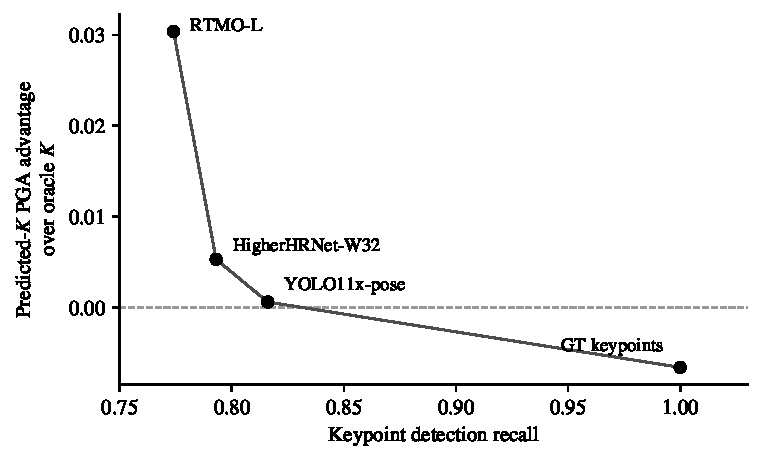
\includegraphics[width=0.75\linewidth]{figures/predk_recall.pdf}
    \caption{Difference in PGA between predicted-$K$ and oracle-$K$
    grouping as a function of keypoint recall for the three detector
    evaluations and the ground-truth-keypoint control. The predicted-$K$
    advantage increases across the three detector operating points as
    recall decreases, while the ground-truth-keypoint control reverses
    the effect when the input is complete. This pattern is consistent
    with the effective-person-count explanation -
    annotation-level $K$ becomes a less appropriate clustering
    constraint as the detected keypoint set becomes less complete.}
    \label{fig:predk_recall}
\end{figure}

The result also clarifies what the K-head's $76.1\%$ exact-count
accuracy does and does not measure.
That figure evaluates the prediction against the annotated number of
people,
whereas the downstream clustering problem operates only on the
keypoints that survived detection and matching.
A prediction counted as incorrect by the former criterion can therefore
still be useful to the latter.
The K-head is not outperforming an oracle estimate of the effective
person count -
rather, it can outperform the annotation-level count when that count
no longer describes the incomplete input to $k$-means.

The autonomous result should therefore not be interpreted as evidence
that estimated counts are generally preferable to known counts.
With complete observations, the ground-truth-keypoint control shows the
opposite.
The result is specific to the detector-based setting,
where the grouping module receives an incomplete representation of the
annotated scene.
In that setting, the predicted count acts as a form of calibration
to the available evidence.
This explains why the autonomous pipeline can slightly outperform the
oracle-$K$ diagnostic while also removing the final ground-truth
dependency from inference.


\subsection{Synthesis}
\label{sec_disc_modularity_autonomy_synthesis}

Reading Sections~\ref{sec_disc_modularity_autonomy_gap}
and~\ref{sec_disc_modularity_autonomy_autonomy} together gives a more
complete picture of the cost and benefit of separating grouping from
detection.
On HigherHRNet detections, the oracle-$K$ PG-GAT pipeline trails the
jointly trained AE reference by $0.0256$ PGA.
In return, the grouping network is no longer tied to the detector that
produced the keypoints.
The detector-swap experiments show that the same frozen PG-GAT
checkpoint can operate on HigherHRNet,
YOLO11x-pose,
and RTMO-L without retraining,
while remaining approximately $0.02$ PGA below each detector's native
grouping.
This is the experimental answer to \emph{RQ3: detector independence},
detector-independent grouping is achievable,
but it carries a small and measurable accuracy cost relative to
detector-specific grouping learned as part of the upstream model.

Whether this trade is worthwhile depends on the intended deployment
setting.
A fixed pipeline in which the detector and grouping mechanism can
always be trained and deployed together has little reason to give up
the additional accuracy of the native grouping method.
The modular design becomes useful when the grouping component must
remain reusable across detectors,
or when detection and grouping need to be developed,
updated,
or deployed independently.
Under those conditions, the approximately $0.020$--$0.022$ PGA
difference measured across the three detectors is the observed cost
of obtaining that flexibility.

The autonomous-pipeline result adds a second dimension to this finding.
Removing the ground-truth $K$ from the inference path might be expected
to introduce another accuracy penalty because errors made by the K-head
can propagate directly into $k$-means.
Instead, the predicted-$K$ HigherHRNet configuration reaches $0.9644$
PGA - compared with $0.9591$ for oracle $K$.
The detector-swap results show the same pattern,
with the predicted-$K$ advantage increasing as keypoint recall decreases.
The ground-truth-keypoint control reverses the effect when the input is
complete.
Taken together, these measurements support the effective-person-count
explanation developed in Section~\ref{sec_disc_modularity_autonomy_autonomy}.

This result changes the role of K estimation in the modular pipeline.
The K-head is not simply an imperfect replacement for information that
would ideally be supplied by an oracle.
In the detector-based setting,
the annotation-level person count and the number of people represented
by the available keypoints can differ.
The K-head operates on the detected representation and can therefore
adapt its prediction to the evidence that actually reaches the grouping
stage.
Its prediction can be wrong relative to the annotated person count
while still providing a better clustering constraint for the incomplete
detection set.

This provides the experimental answer to \emph{RQ7: autonomous
deployment}.
The final pipeline does not require ground-truth person counts at
inference,
and removing that dependency does not reduce the measured grouping
accuracy on the detector outputs tested here.
For HigherHRNet and RTMO-L it improves it measurably,
while for YOLO11x-pose the difference is close to neutral.
The ground-truth control is equally important to this conclusion -
it shows that predicted $K$ is not intrinsically superior to known $K$,
but becomes useful when detection errors create a mismatch between the
annotated scene and the evidence presented to the grouping algorithm.

The combined result is therefore stronger than the oracle-$K$
modularity experiment alone.
PG-GAT pays a modest accuracy cost to separate grouping from detection,
and the detector-swap experiments show that this separation is
operational across multiple detector families.
The K-head then removes the remaining ground-truth dependency without
introducing the expected additional penalty and,
under incomplete detection, can partially offset the oracle-$K$
grouping cost.
The contribution is consequently not that modularity is free,
but that its cost is measured,
stable across the detectors tested,
and compatible with a fully autonomous inference pipeline.